\section{Detailed design description}
Die schon gezeigten Module besitzen folgende I/Os:
\begin{figure}[!ht]
 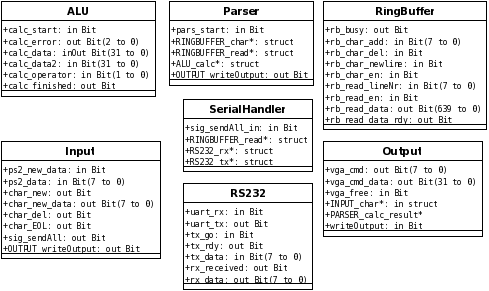
\includegraphics[scale=0.7]{pics/Klassen.png}
 % Modules.png: 501x145 pixel, 72dpi, 17.67x5.12 cm, bb=0 0 501 145
 \label{fig:Klassen}
\end{figure}

% \begin{itemize}
% \item Description how the design will be implemented
% \item Event sequence digrams
% \item Internal structure
% 	\begin{itemize}
% 	\item Memory
% 	\item Logic blocks
% 	\item Parallel processes
% 	\item State machines
% 	\end{itemize}
% \end{itemize}
\subsection{ALU}
Die Alu führt nach dem Startsignal die am \textit{operation}seingang gewählte 
Rechenoperation ausgeführt. Dazu stehen folgende Optionen am operationseingang zur Verfügung:
\begin{center}
% use packages: array
\begin{tabular}[!ht]{|l|l|l|}
\hline Eingang (binär) & Rechenoperation & Rechnungsart\\ 
	00 & Addieren & Strichrechnung\\ 
	01 & Subtrahieren & Strichrechnung\\ 
	10 & Multiplizieren & Punktrechnung\\ 
	11 & Dividieren & Punktrechnung\\
 \hline
\end{tabular}
\end{center}
Die division schneidet nachkommastellen ab.
Die dafür benötigten Fälle werden anhand von cases unterschieden.
\subsection{Parser}
Den Parser arbeitet mit zwei Integer Puffern. \\
Nach starten des Parsers werden sukzessive alle sich in einer Zeile befindenden CHARs durchgearbeitet.

wird die erste Zahl gefiltert und in den \textit{Punktrechnungsbuffer} geschoben.
Folgt eine
\subsection{Ringbuffer}
Ringbuffer Funktionalitäten:
\begin{itemize}
 \item Hinzufügen eines CHARs zu der aktuellen Zeile
 \item Löschen des letzten CHARs der aktuellen Zeile
 \item Wechseln in die nächste Zeile
 \item Auslesen einer gesamten Zeile mit konkreter Nummer
 \item Ressource blockierbarkeit
\end{itemize}
Aktuelle Zeile des Ringbuffers wird immer mit dem Wert 0 gekennzeichnet.

\subsection{RS232}
Das RS232 Modul überwacht die Empfangsleitung und stellt nach Empfang die Daten auf einem 
8 Bit Bus zur Verfügung.\\
Beim Senden bezieht es 8 Bit von dem Eingangsbus und meldet den Versandt über ein ready Bit.

Beide Modi arbeiten mit 8 Datenbits, einem Stopbit und keinem paritätsbit, bei einer
Boudrate von 115`200
%Senden: TX->LOW alle 8.68us nächstes Bit, dann 1 zum Stoppen
\subsection{Input}
Input arbeitet die vom ps/2 Modul empfangenen Daten ab und sendet diese je nach Empfangsdaten weiter.\\
Unterscheidung der Empfangenen Daten:
\begin{description}
 \item[0-9,+,-,*,/] 
	\begin{itemize}
		\item Wandeln der Scancodes in ASCII chars 
		\item Speichern der Chars im RingBuffer
		\item Senden der Chars an den Output
	\end{itemize}
 \item[Enter] Senden an Parser und Output
 \item[Backspace] Senden an RingBuffer und Output
 \item[Space] Senden an RingBuffer und Output
 \end{description}

Des Weiteren überwacht das Input Modul einen Button am development Board und sendet
daraufhin eine Anfrage an den SerialHandler
\subsection{Output}
Das output Modul verarbeitet die vom \textit{Input} und \textit{Parser} erhaltenen Daten indem er sie an das VGA-Modul schickt.